\subsection{Autoencoder}

The idea of the approach is to use a low-dimensional version of the data to identify anomalies either using a trained model or the reconstructing error when reconstructing the encoded data.
The approach from \cite{cf_AE} consists of two stages. 
Firstly, the dimension of the high-dimension credit card data is reduced using an undercomplete \acfi{AE}, which is a feed-forward neural network depicted in \autoref{fig:AE_Aufbau} that learns efficient (non-correlated) encodings for the input data. It is called undercomplete because the dimension of its hidden layer, or so-called latent space, is smaller than the dimension of the input layer. Feed-forward means that after training the information moves in only one direction (forward) and thus, no loops or cycles exist. However, while training, the network employs backpropagation\footnote{updating weights and biases of the neurons based on forward propagation error} to update the parameters.
%
\begin{figure}[http]
    \begin{center}
      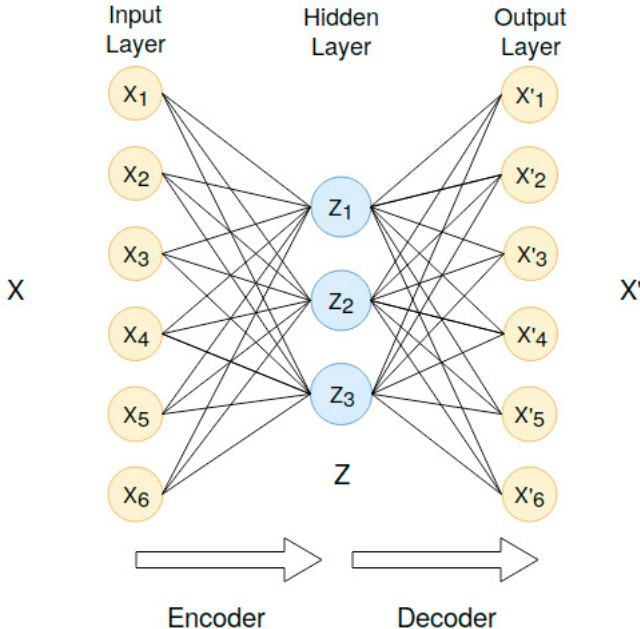
\includegraphics[scale=0.3]{images/AE_Aufbau.jpg}
      \caption{Structure of \ac{AE} from \cite{cf_AE}}
      \label{fig:AE_Aufbau}
    \end{center}
\end{figure}

The goal of an \ac{AE} is to approximate the identity function $f_\theta(X) = X$ (trivial solution eliminated) for input $X$ and function parameters to be learned $\theta$.
The input and output layer have the same dimension since the encoded data is reconstructed in the output layer. 

The mathematical background of the encoder is given in \eqref{eq:encoder}. The dimension reduction is computed using weight $W_\theta$, bias $B_\theta$ of the encoder layer, and the (non-)linear encoder activation function $f_E(.)$. Owing to the usage of a non-linear activation function, the neural network is capable of more than linear regression.
%
\begin{ceqn}
    \begin{equation}
    \label{eq:encoder}
        Z = f_E(W_\theta X + B_\theta)
    \end{equation}
\end{ceqn}
%
The decomposition of the reduced dimensionality data to the output $X'$ is calculated analogously to \eqref{eq:encoder}. \eqref{eq:decoder} is used for the decoder.
%
\begin{ceqn}
    \begin{equation}
    \label{eq:decoder}
        X' = f_D(W_\theta Z + B_\theta)
    \end{equation}
\end{ceqn}
%
The Euclidean distance from \eqref{eq:recon_err} between the input $X$ and the output $X'$, which is reconstructed from $Z$, is considered the reconstruction error. According to \cite{AE_RF}, error backpropagation and gradient descent\footnote{iterative algorithm to find the function’s coefficients that minimise the corresponding cost function using derivatives and the learning rate} are employed to train the \ac{AE} with the goal of minimising the reconstruction error. The reconstruction error can be used to identify anomalies: If the reconstruction error is greater than a certain threshold\footnote{e.g. iterative computation of the threshold value analogously to \autoref{alg:AE_PRF}}, $X$ is considered an anomaly based on the hypothesis that the \ac{AE} has approximated the identity function for normal instances.
%
\begin{ceqn}
    \begin{equation}
    \label{eq:recon_err}
       \triangle (X, X') = \parallel X - X' \parallel_2
    \end{equation}
\end{ceqn}
%
To avoid overfitting, a regulariser tuning the objective function of the learning algorithm may be added.

The approach from \cite{cf_AE} first uses the encoder, which transforms $X$ to $Z$. Since the authors assume that $X$ can be reconstructed using $Z$, it is a valid representation of the input transaction.
Then, a classifier is trained on $Z$. In \cite{cf_AE} labelled transactions of a training set are used to train a \acfi{MLP}, \acfi{kNN}, \acfi{LR}, but generally, every model can be used to identify anomalies. 
%
\begin{algorithm}
\caption{\acfi{AE-PRF}}\label{alg:AE_PRF}
 \hspace*{\algorithmicindent} \textbf{Input:} training data $D_{train}$,  validation data $D_{val}$, test data $D_{test}$, metric $M$ \\
 \hspace*{\algorithmicindent} \textbf{Output:} classification of each instance (0 if normal, 1 else)

\begin{algorithmic}[1]
\State Train the \ac{AE} model $\ac{AE}_T$ with $D_{train}$
\Comment{pseudocode based on \cite{AE_RF}}
\State $T \gets \ac{AE}_T(D_{train})$
\Comment{$T$ set of training data after dimension reduction}
\State Train the \ac{RF} model $\ac{RF}_T$ with $T$
\State $V \gets \ac{AE}_T(D_{val})$
\Comment{$V$ set of validation data after dimension reduction}
\For{$\theta \gets 0$ \texttt{to} $1$ \texttt{step} $0.01$}
\Comment{iterative testing of possible threshold values $\theta$}
    \For{$v \in V$}
        \State $p \gets \ac{RF}_T(v)$
        \Comment{probability $p$ of fraud classification}
        \If{$p > \theta$} 
            \State \texttt{result}$[\theta][v] \gets 1$
        \Else
            \State \texttt{result}$[\theta][v] \gets 0$
        \EndIf 
    \EndFor
\EndFor

\State Find best $\theta*$ by comparing all \textit{result} values in terms of metric $M$
\State $C \gets \ac{AE}_T(D_{test})$
\Comment{$C$ set of test data after dimension reduction}

 \For{$c \in C$}
        \State $q \gets \ac{RF}_T(c)$
        \If{$p > \theta*$} 
            \State \texttt{output}$[c] \gets 1$
        \Else
            \State \texttt{output}$[c] \gets 0$
        \EndIf 
    \EndFor

\State \textbf{return} \textit{output}
\end{algorithmic}
\end{algorithm}
%

\cite{AE_RF} proposes an \acfi{AE-PRF}, which is the combination of an \ac{AE} to extract transaction data features and a \ac{RF} with probabilistic classification to assign either the label fraudulent or normal to credit card transactions.
The approach \ac{AE-PRF} is illustrated in pseudocode in \autoref{alg:AE_PRF}.
The \ac{RF} in the paper is an ensemble learning model consisting of \acp{DT} and employs bagging\footnote{independently training multiple individual \acp{DT} based on random subsets of data and attributes}. In this case the \acp{DT}' internal nodes split the data set on the optimal (i.e. largest information gain) value of the corresponding split attribute. 
The splitting terminates if either all data of a node have the same value, the number of instances at a node reaches a predefined minimum limitation or the depth of the node reaches a predefined maximum limitation.
An instance is then passed through the tree and classified by an individual tree based on the label of its corresponding leaf. The final \ac{RF} classification of that instance is the result of a majority voting or averaging of the individual \acp{DT}, which have been constructed prior by using bagging.
The probabilistic classification requires an additional parameter threshold $\theta \in  [0,1]$. The \ac{RF} model classifies an instance as fraudulent with probability $p$ and respective as normal with probability $1 - p$. 
The final \ac{AE-PRF} classification of that instance is fraudulent if $p > \theta$ is true and normal otherwise.
The optimal threshold $\theta*$ can be determined by iterative testing of the classification performance in terms of a specific metric $M$ on different values for $\theta$.
